\documentclass[english,svgnames,notes=hide,12pt]{beamer}
\usepackage{macros-ohp}
\usepackage{graphicx}

\newcommand*{\pardus}{%
\item[{\includegraphics[width=0.6cm]{imgs/pardus}}]%
    }

\newcommand*{\ubuntu}{%
\item[{\includegraphics[width=0.6cm]{imgs/ubuntu}}]%
    }

\newcommand*{\debian}{%
\item[{\includegraphics[width=0.6cm]{imgs/debian}}]%
    }

\newcommand*{\redhat}{%
\item[{\includegraphics[width=0.6cm]{imgs/redhat}}]%
    }
\newcommand*{\suse}{%
\item[{\includegraphics[width=0.6cm]{imgs/suse}}]%
    }

\newcommand*{\gentoo}{%
\item[{\includegraphics[width=0.6cm]{imgs/gentoo}}]%
    }

\newcommand*{\raspi}{%
\item[{\includegraphics[width=0.6cm]{imgs/raspi}}]%
    }

\newcommand*{\centos}{%
\item[{\includegraphics[width=0.6cm]{imgs/centos}}]%
    }

\newcommand*{\mint}{%
\item[{\includegraphics[width=0.6cm]{imgs/mint}}]%
    }





\def\seminarname{Özgür Yazılım}
\def\presentationtitle{II. Pardus ve Açık Kaynak Günleri, Samsun}

\title{\large\seminarname:\\\large\presentationtitle}
\author{Mustafa Karakaplan\\
    \small İnönü Üniversitesi, Malatya
}

% Fill the date or leave it blank to not display it
\date{24-26 Nisan 2019}

\begin{document}
\thispagestyle{empty}
%\begin{frame}[plain] %put [plain] at the end to get rid of the page number on this page
\begin{frame}
    \titlepage
\end{frame}

\begin{frame}
    \frametitle{Konular}
    \tableofcontents
\end{frame}


\section{Özgür Yazılım}

\begin{frame}
\frametitle{Özgürlük Nedir? (TDK)}

\begin{enumerate}[<+->]
\item  Herhangi bir kısıtlamaya, zorlamaya bağlı olmaksızın düşünme veya davranma, herhangi bir şarta bağlı olmama durumu, serbestî\\
~\\
\item Her türlü dış etkiden bağımsız olarak insanın kendi iradesine, kendi düşüncesine dayanarak karar vermesi durumu, hürriyet
\end{enumerate}

\end{frame}

\begin{frame}
\frametitle{Bazı Tüketicilere Göre Özgür Yazılım}
\begin{itemize}[<+->]
    \item Para vermeden sahip olmaktır.
    \item Crack i bulunan yazılım demektir.
    \item Kopyasını satabilmektir.
    \item Bir oyunu kırıp sonsuz hile kazanabilmektir. 
    \item Yazılıma para vermeden para kazanabilmektir.
    \item Değiştirip kendi markasıyla pazarlayabilmektir. 
\end{itemize}
\end{frame}

\begin{frame}
\includegraphics[width=1.0\textwidth]{imgs/software_wars}

\end{frame}


\begin{frame}
\frametitle{Özgür yazılımlarda 4 temel özgürlüğün bulunması gerekir}

\begin{enumerate}[<+->]
\setcounter{enumi}{-1}
\item Herhangi bir amaç için yazılımı çalıştırma özgürlüğü.
\item Her ne yapılmak isteniyorsa, programın nasıl çalıştığını öğrenmek ve onu değiştirme özgürlüğü, Bu özgürlük aynı zamanda yazılımın kaynak koduna ulaşabilmeyi de gerektirir.
\item Kopyaları dağıtma özgürlüğü, böylece başkalarına yardım edebilirsiniz.
\item Toplumun yarar sağlayabileceği biçimde yazılımı geliştirme ve geliştirilen yazılımı yayınlama özgürlüğü.
\end{enumerate}
\end{frame}

\section{Lisans Modelleri}
\begin{frame}
\frametitle{Lisans Modelleri}
\begin{itemize}[<+->]
    \item Sahipli Yazılım, Ticari Yazılım
    \item GNU "GNU is not Unix"
    \item COPYLEFT (Telif Feragatı)
   \item GNU Genel Kamu Lisansı (GPL)
   \item GNU Kısıtlı Genel Kamu Lisansı (LGPL)
   \item MIT ve BSD lisansları
\item FreeWare (Ücretsiz Sahipli Yazılım), ShareWare (Kısıtlı Yazılım)
\item Kamuya Açık Yazılım
\end{itemize}
\end{frame}



\begin{frame}
\frametitle{Özgür Yazılım Ne Sağlar?}
\begin{itemize}[<+->]
    \item Yazılımın kalitesini artırır.
    \item Yazılımın çeşitlenmesine olanak sunar.
  \item Yazılım geliştirme kapasitesi artar.
    \item Yerelleştirme, Sonsuz seçme özgürlüğü sunar.
   \item Hızlı güncelleme olanağı sunar.
   \item Hatalar çabuk giderilir.
   \item Ortak çalışabilirlik sunar. Her şey şeffaftır.
 \item Telif hakkı ihlalleri azalır. Standartlar oluşmasını sağlar. 
\end{itemize}
\end{frame}

\begin{frame}
\frametitle{Özgür Yazılımın Ekonomik Faydaları}
\begin{itemize}[<+->]
    \item Toplam sahip olma maliyeti azalır.
    \item Rekabetin artırılması, tekelleşmeyi engelleme.
  \item Donanım yaşam süresini artırır.
    \item İş verimliliğini artırır.
   \item Daha güvenli ulusal ve kurumsal güvenlik.
   \item Tedarikçi ortadan kalkar.
 \item Dışa bağımlılık azalır. 
\end{itemize}
\end{frame}




\section{Linux Dağıtımları}

\begin{frame}
\frametitle{Linux}
\begin{columns}
\begin{column}{0.6\textwidth}
Linux; bilgisayar işletim sistemlerinin en temel parçası olan çekirdek yazılımlarından bir tanesidir. GNU Genel Kamu Lisansı ile sunulan ve Linux Vakfı çatısı altında geliştirilen bir özgür yazılım projesidir. Linux ismi ilk geliştiricisi olan Linus Torvalds tarafından 1991 yılında verilmiştir.
\end{column}

\begin{column}{0.4\textwidth}
\includegraphics[width=0.6\textwidth]{imgs/linus}
\end{column}

\end{columns}

\end{frame}


\begin{frame}
\frametitle{Pardus}
\begin{columns}
\begin{column}{0.5\textwidth}
Pardus, Türkiye'de TÜBİTAK tarafından geliştirilen bir Linux dağıtımı olan işletim sistemi. Planlamasına 2003 yılında başlanmış olup ilk kararlı sürümü 27 Aralık 2005’te yayınlanmıştır. Pardus adı, Anadolu Parsı'nın bilimsel adı olan Panthera pardus tulliana'dan gelmektedir.
\end{column}

\begin{column}{0.5\textwidth}
\includegraphics[width=1.0\textwidth]{imgs/pardusl}
\end{column}

\end{columns}

\end{frame}







\begin{frame}
\frametitle{Top 500 Süper Bilgisayar}
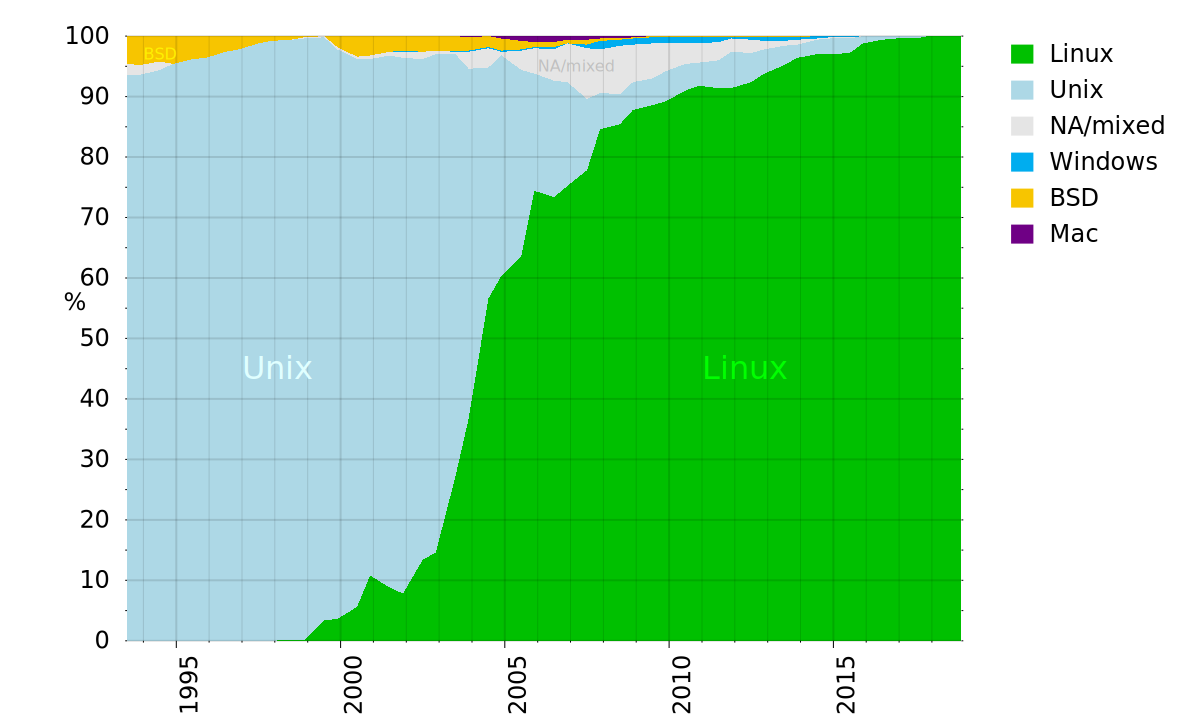
\includegraphics[width=1.0\textwidth]{imgs/top500}

\end{frame}


\begin{frame}
\frametitle{Linux Kullanımı}
\begin{columns}
\begin{column}{0.5\textwidth}
\textbf{Bilgisayarlarda}\\
~\\

\begin{tabular}{lr}
İşletim Sistemi & Yüzde \\
\hline
Windows & 87.45 \\
Mac OS  & 9.73  \\
Linux   &  2.16 \\
Chrome OS & 0.33 \\
\end{tabular}
\end{column}

\begin{column}{0.5\textwidth}
\textbf{Mobil Cihazlarda}\\
~\\

\begin{tabular}{lr}
Platform & Yüzde \\
\hline
Android (Linux) & 70.21 \\
IOS  & 28.24  \\
Windows & 0.09 \\
\end{tabular}

\end{column}

\end{columns}

\end{frame}




\begin{frame}
\frametitle{Linux Dağıtımları}
\begin{itemize}[<+->]
  \debian Debian, Debian Project
    \pardus Pardus, TÜBİTAK
    \ubuntu Ubuntu, Canonical
    \mint Mint,  Linux Mint Community
\raspi Raspbian, Raspberry Pi Foundation
    \redhat RedHat, RedGat Inc.
\gentoo Gentoo, Gentoo Foundation
\centos Centos, The Community ENTerprise Operating System 
\end{itemize}
\end{frame}

\begin{frame}
\frametitle{Masaüstü Ortamı}

\begin{itemize}[<+->]
\item GNOME
\item KDE Plasma
\item Cinnamon
\item Unity
\item Xfce
\item LXDE/LXQt
\item MATE 
\end{itemize}
\end{frame}

\begin{frame}
\frametitle{Özgür - Açık Kaynak Yazılımlar}
\begin{tabular}{rl}
Ofis, MUY & LibreOffice,  \LaTeX{}, Scribus\\
Web tarayıcı &Google Chrome, Mozilla Firefox\\
Medya Oynatma &VLC, MPlayer\\
Video İşleme & OpenShot, Ffmpeg \\
Resim, Vektörel& Gimp, Inkscape, Dia, GraphViz\\
CAD, Elektronik  &FreeCAD, LibreCAD, KiCAD\\
	3D, Anim, Oyun & Blender, Godot, Cocos2d-x, Spring, Panda 3D  \\
İndirme Araçları & Transmission, Axel, Wget\\ 
Programlama & OpenJDK, GCC, Python, ...\\ 
\end{tabular}
\end{frame}


\section{Kaynaklar}
\begin{frame}
    \frametitle{Kaynaklar}
https://www.pardus.org.tr\\
https://opensource.com\\
https://www.gnu.org \\
~\\
~\\
	Bu sununun pdf dosyasına ve \LaTeX{} kaynak koduna \\
~\\
\href{https://github.com/karakaplanm/sunu}{https://github.com/karakaplanm/sunu}

~\\
adresinden erişebilirsiniz.

\end{frame}

\end{document}



